\begin{multicols}{2}

\usetikzlibrary{shapes,positioning}

\newcommand{\foo}{\hspace{-2.3pt}$\bullet$ \hspace{5pt}}

\raggedright
\newcounter{year2}
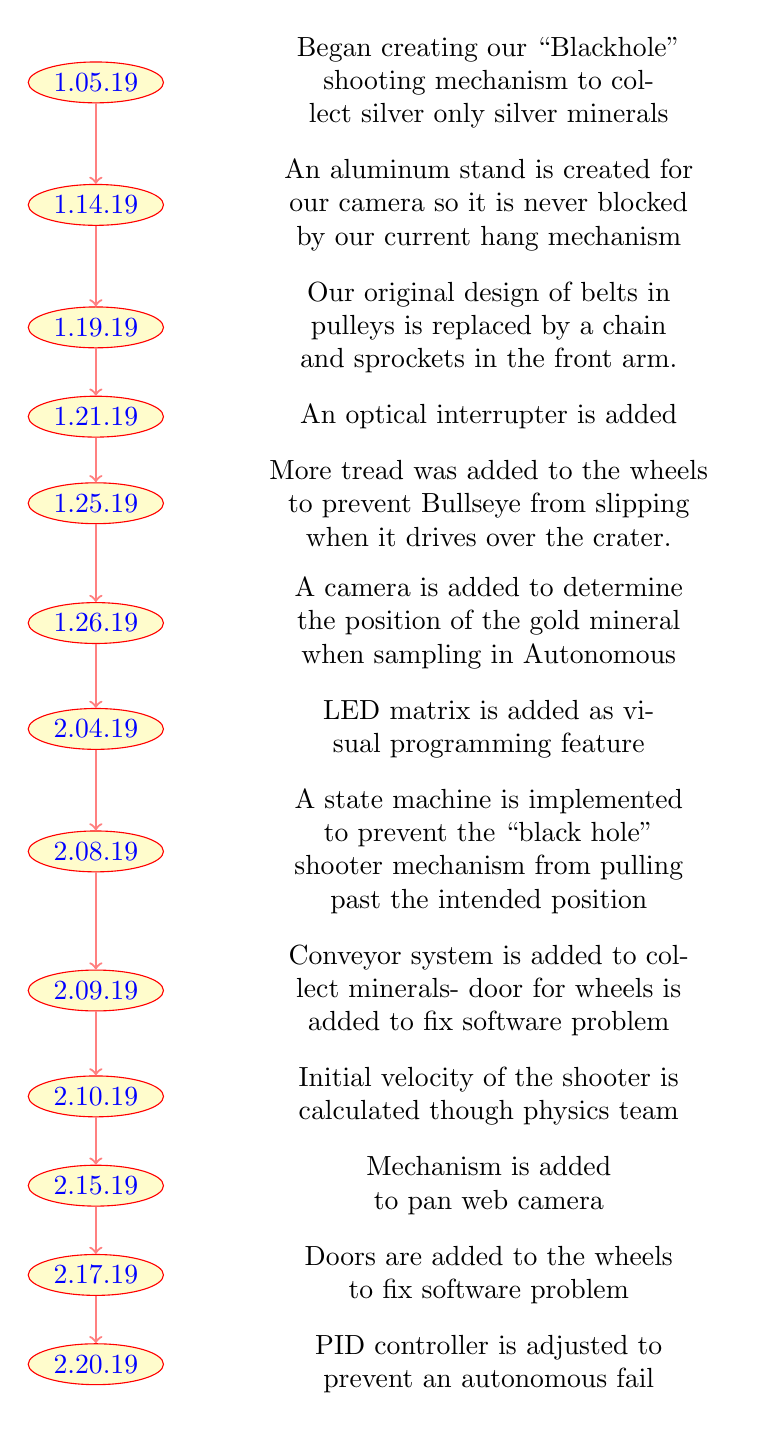
\begin{tikzpicture}[yscale=0.5,%
           year2/.style={draw=red,text=blue,fill=yellow!20,shape=ellipse,inner sep=2pt},
           description/.style={rectangle,align=center,text width=60mm,anchor=west},
           timeline/.style={->,thick,red!50}]

    \foreach \year/\desc [count=\y] in {%
       1.05.19/Began creating our “Blackhole” shooting mechanism to collect silver only silver minerals,%
       1.14.19/An aluminum stand is created for our camera so it is never blocked by our current hang mechanism,%
       1.19.19/Our original design of belts in pulleys is replaced by a chain and sprockets in the front arm.,%
       1.21.19/An optical interrupter is added,%
       1.25.19/More tread was added to the wheels to prevent Bullseye from slipping when it drives over the crater.,%
       1.26.19/A camera is added to determine the position of the gold mineral when sampling in Autonomous,%
       2.04.19/LED matrix is added as visual programming feature,%
       2.08.19/A state machine is implemented to prevent the “black hole” shooter mechanism from pulling past the intended position,%
       2.09.19/Conveyor system is added to collect minerals- door for wheels is added to fix software problem,%
       2.10.19/Initial velocity of the shooter is calculated though physics team,%
       2.15.19/Mechanism is added to pan web camera,%
       2.17.19/Doors are added to the wheels to fix software problem,%
       2.20.19/PID controller is adjusted to prevent an autonomous fail%
       } { \ifnum\y=1 \node[description](\y){\desc};
           \else\node[description,below=1ex of \z](\y){\desc};
           \fi
           \node[year2](y-\y) [left=of \y] {\year};
           \ifnum\y>1\draw[timeline] (y-\z)-- (y-\y);\fi
           \global\let\z=\y% for drawing from last node
       }


\end{tikzpicture}

\columnbreak

\raggedleft
\begin{center}
        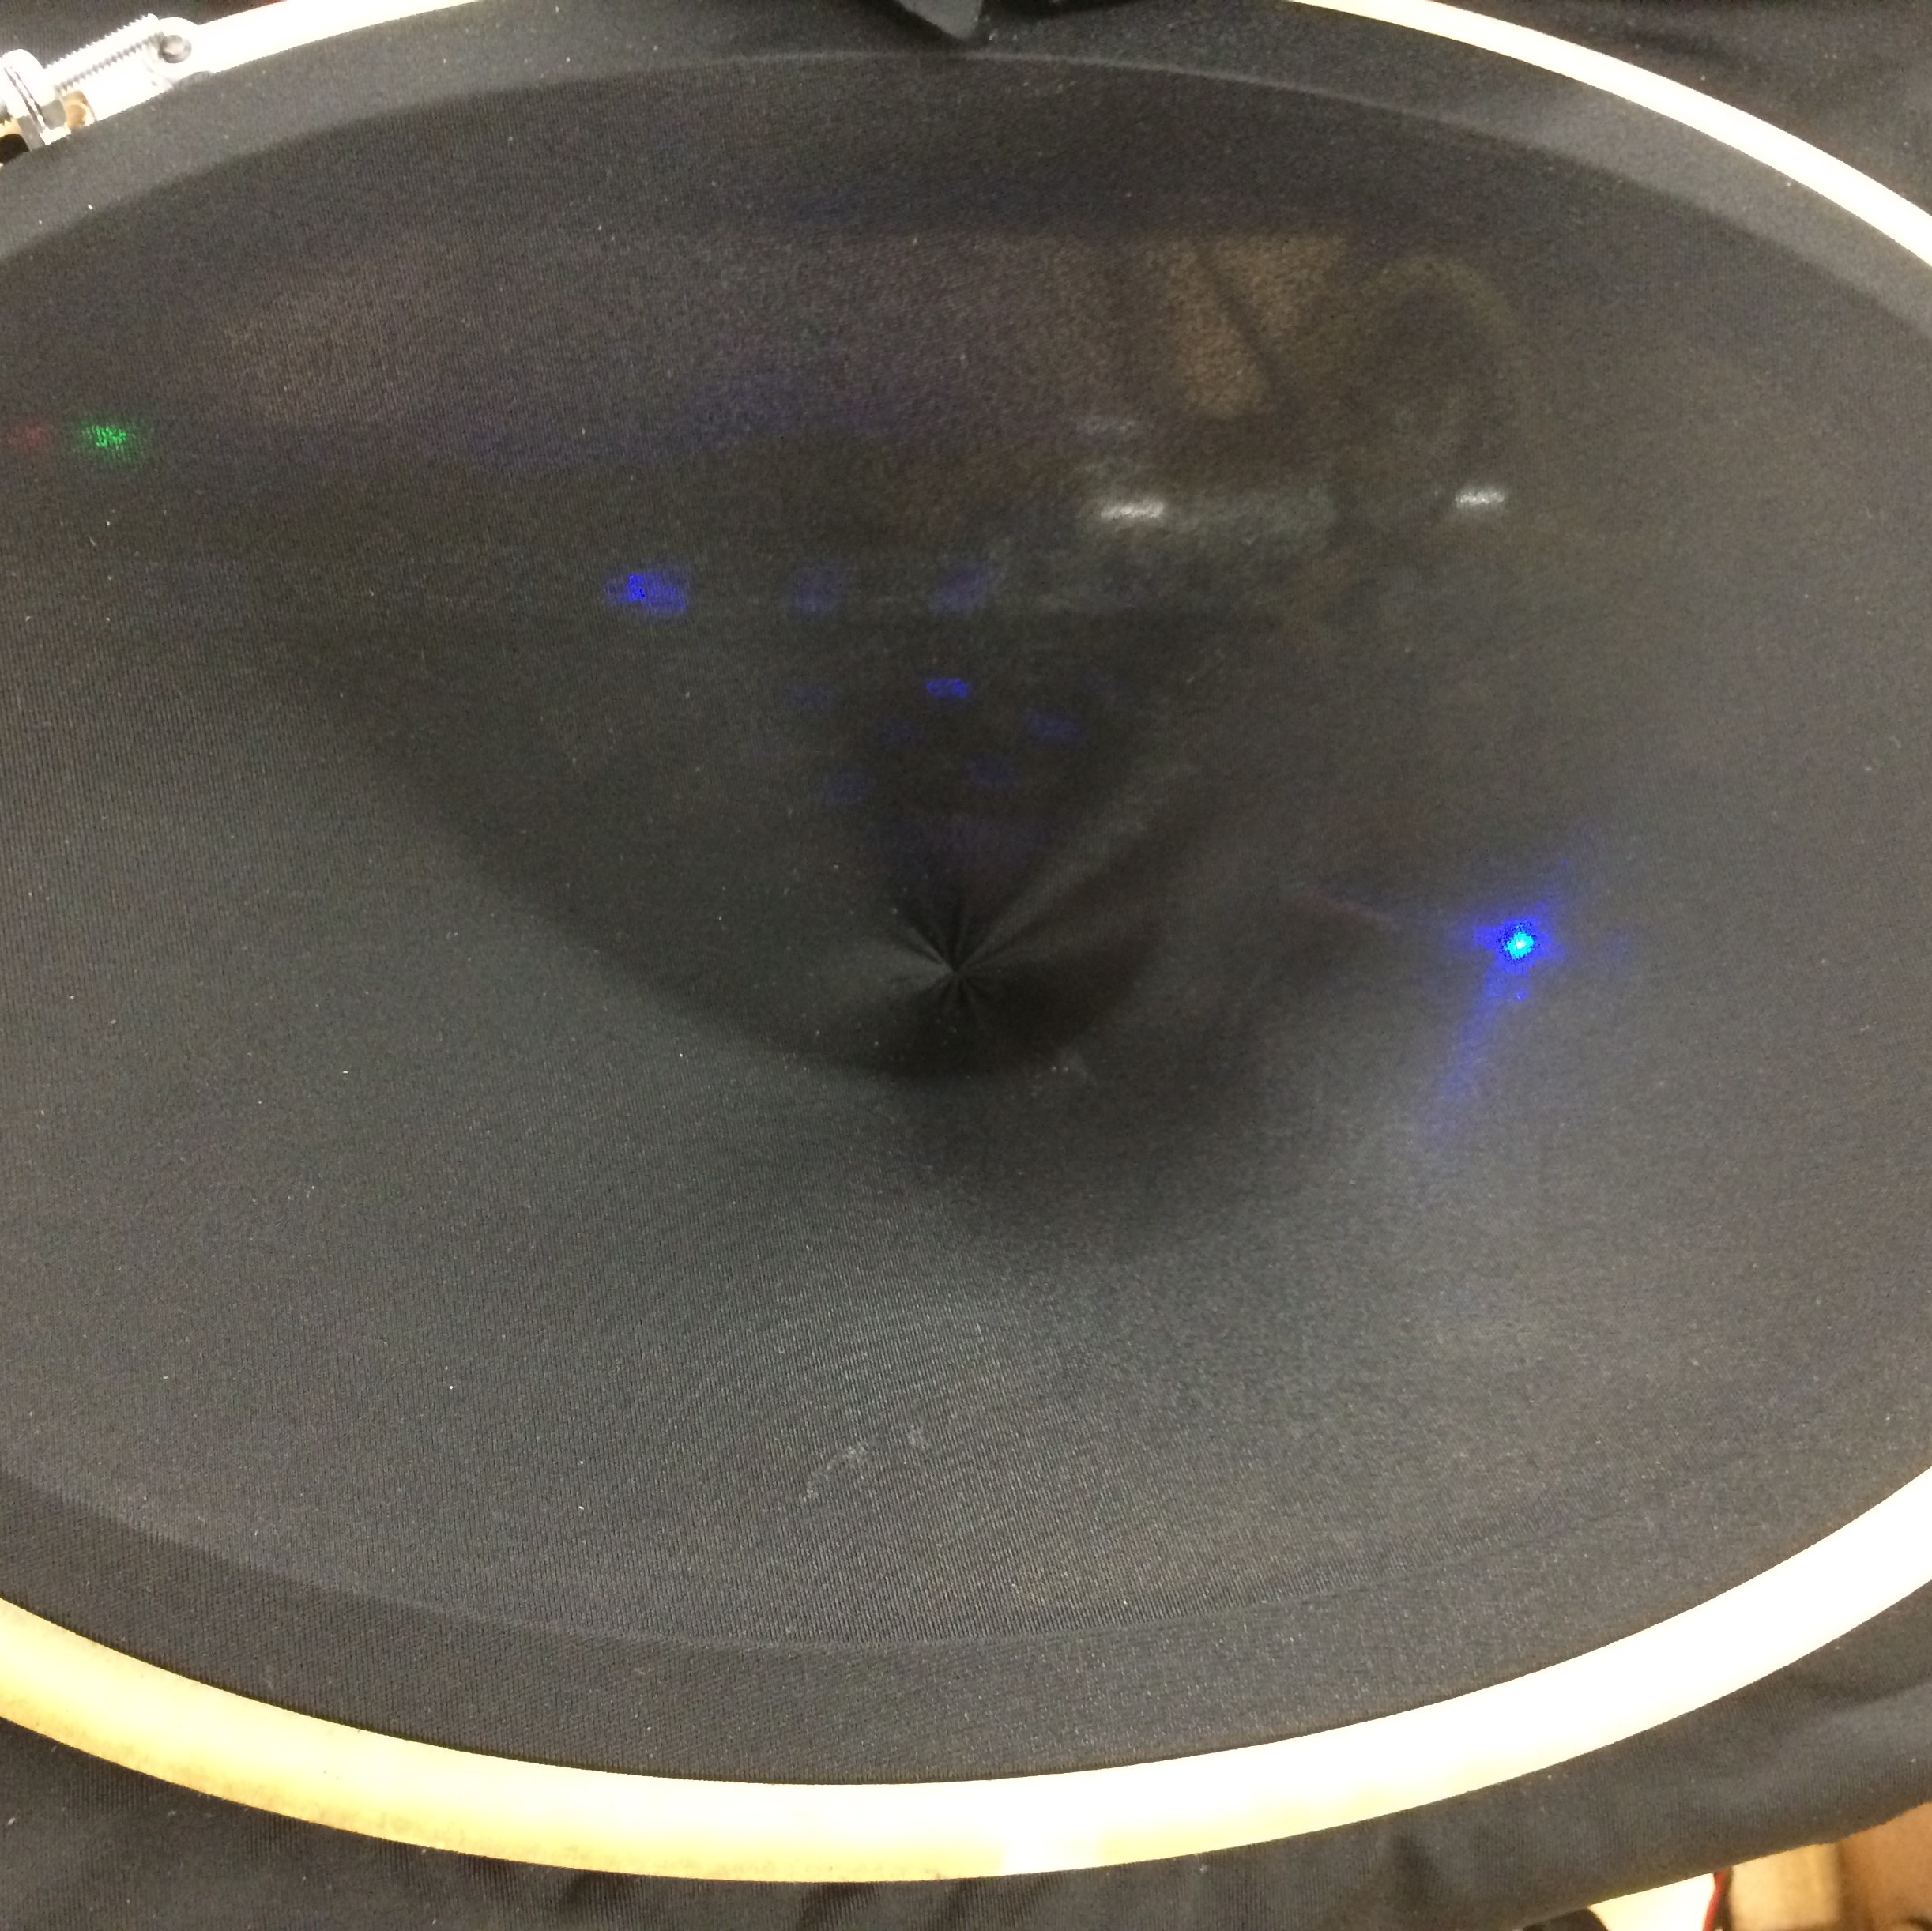
\includegraphics[width=.13\textwidth]{Design_Overview/timephoto11.jpg}
\end{center}
\begin{center}
        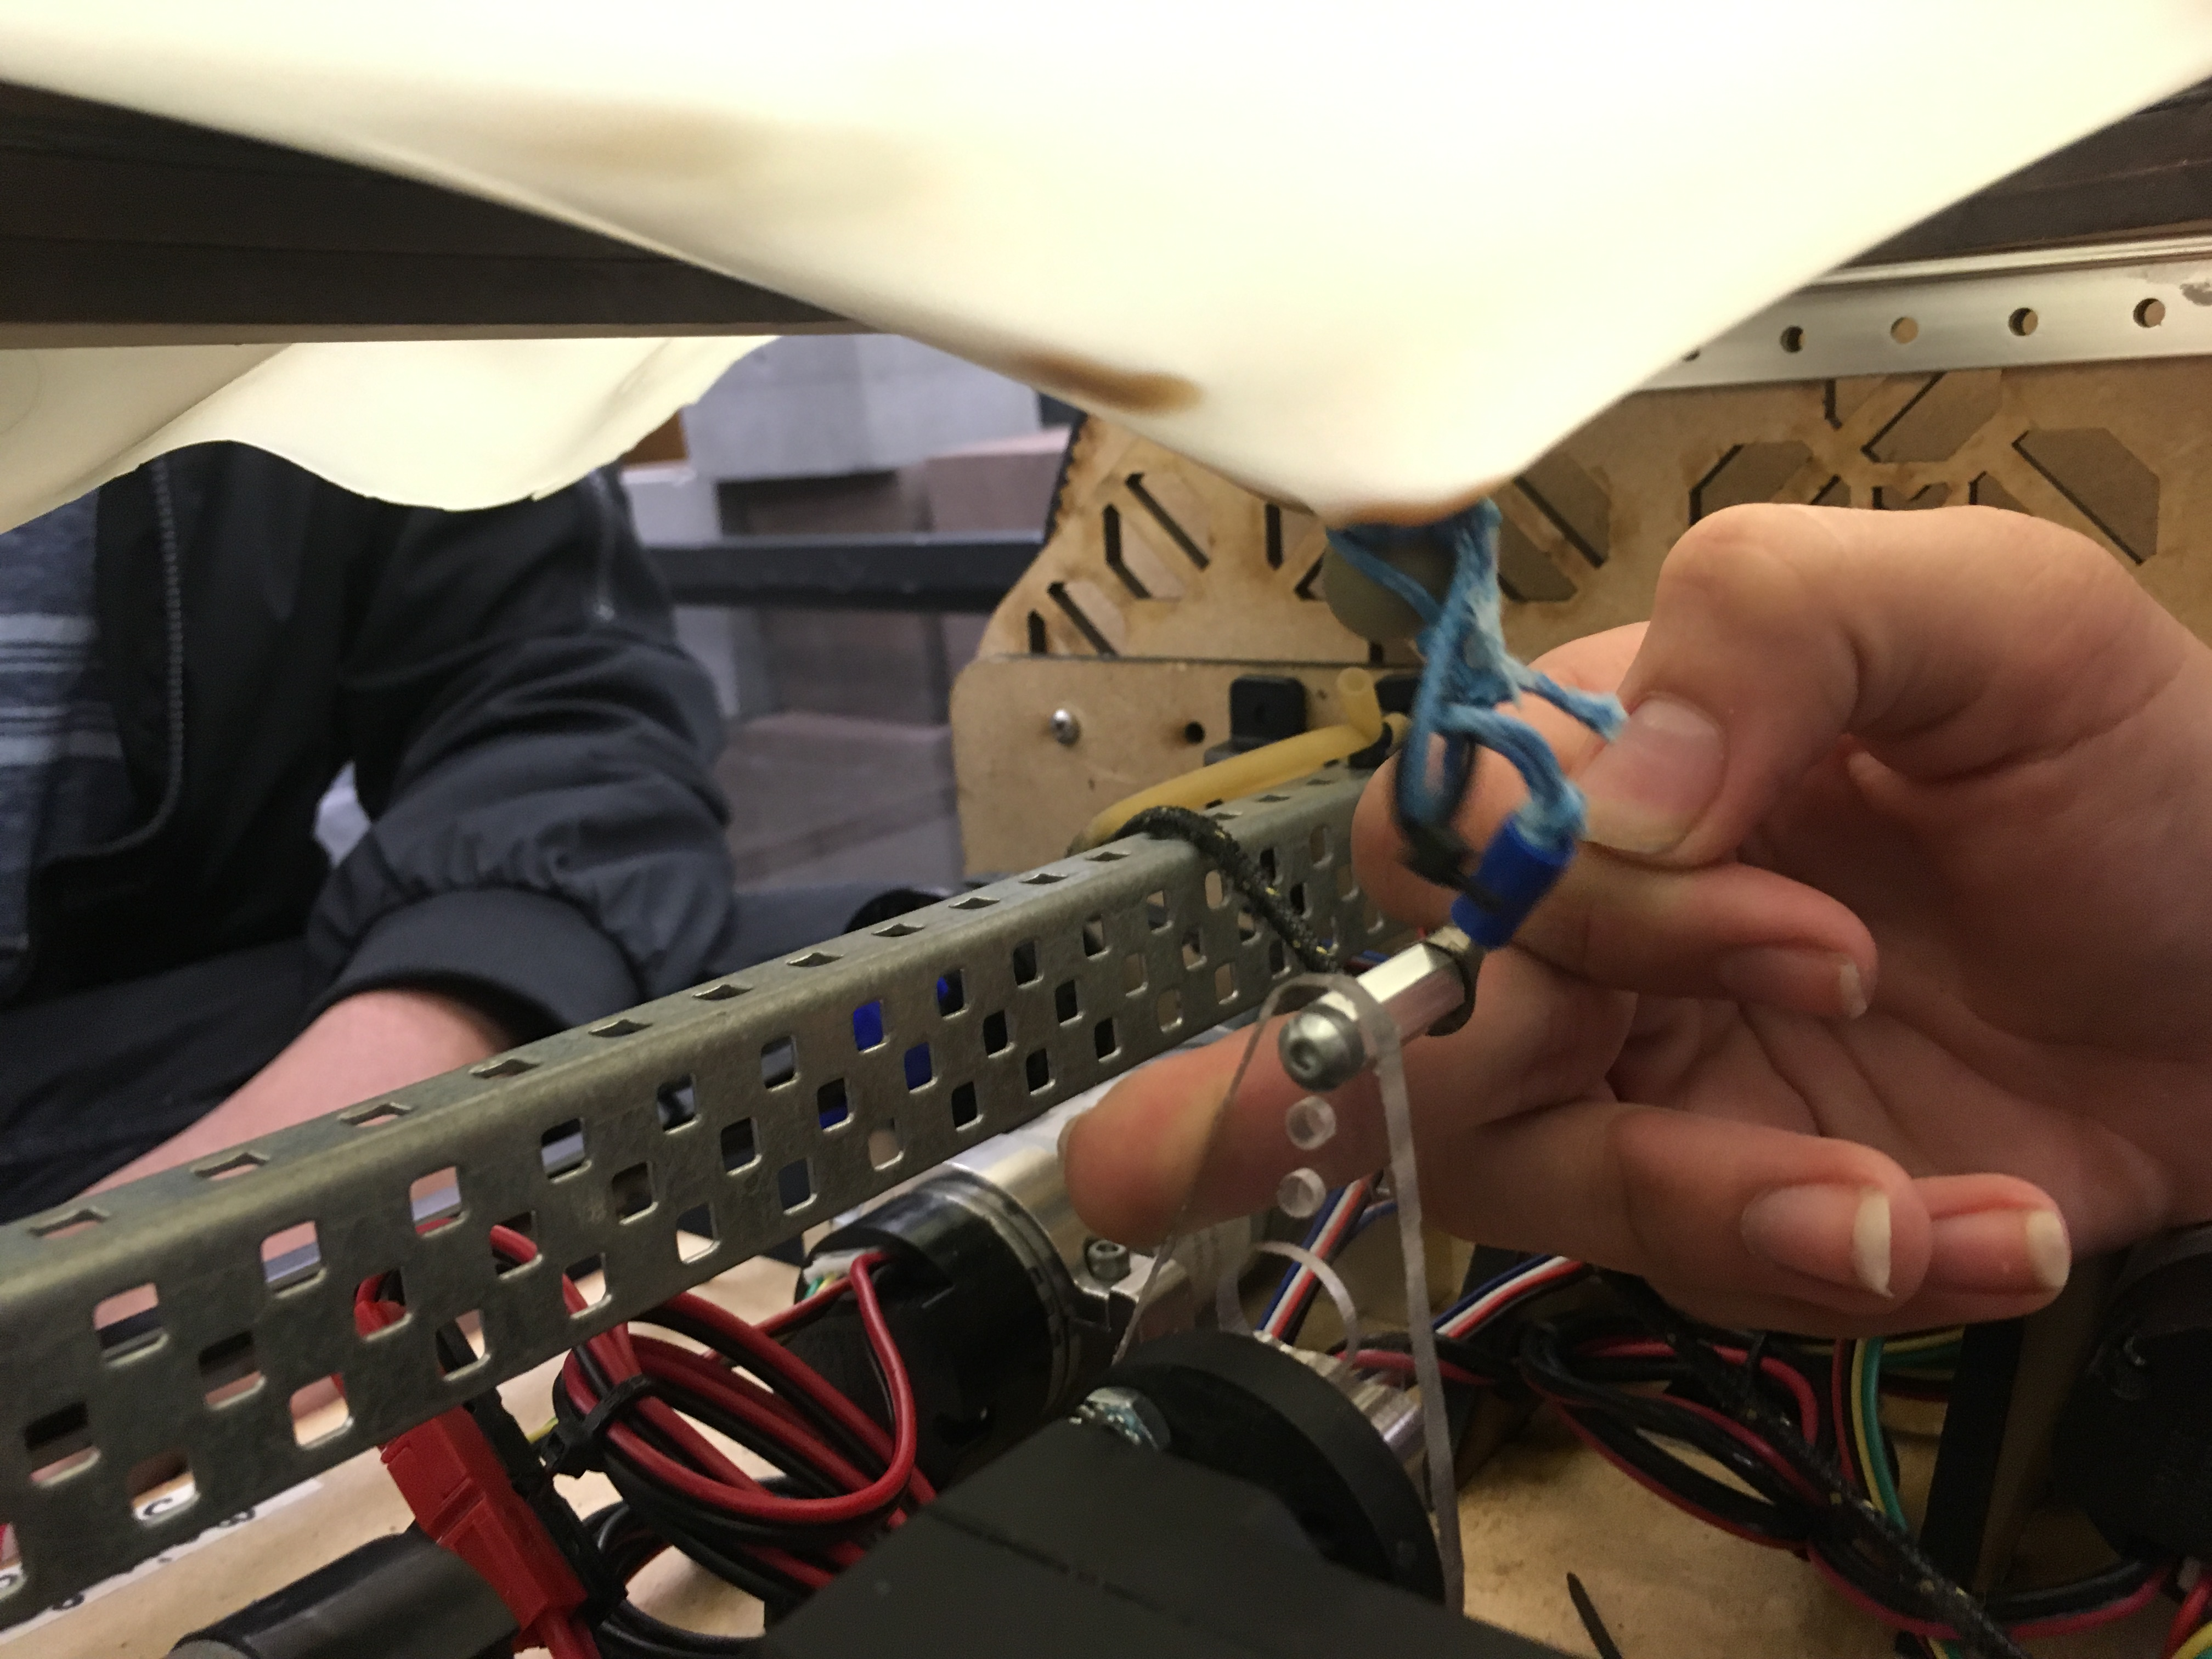
\includegraphics[width=.13\textwidth]{Design_Overview/timephoto12.JPG}
\end{center}
\begin{center}
        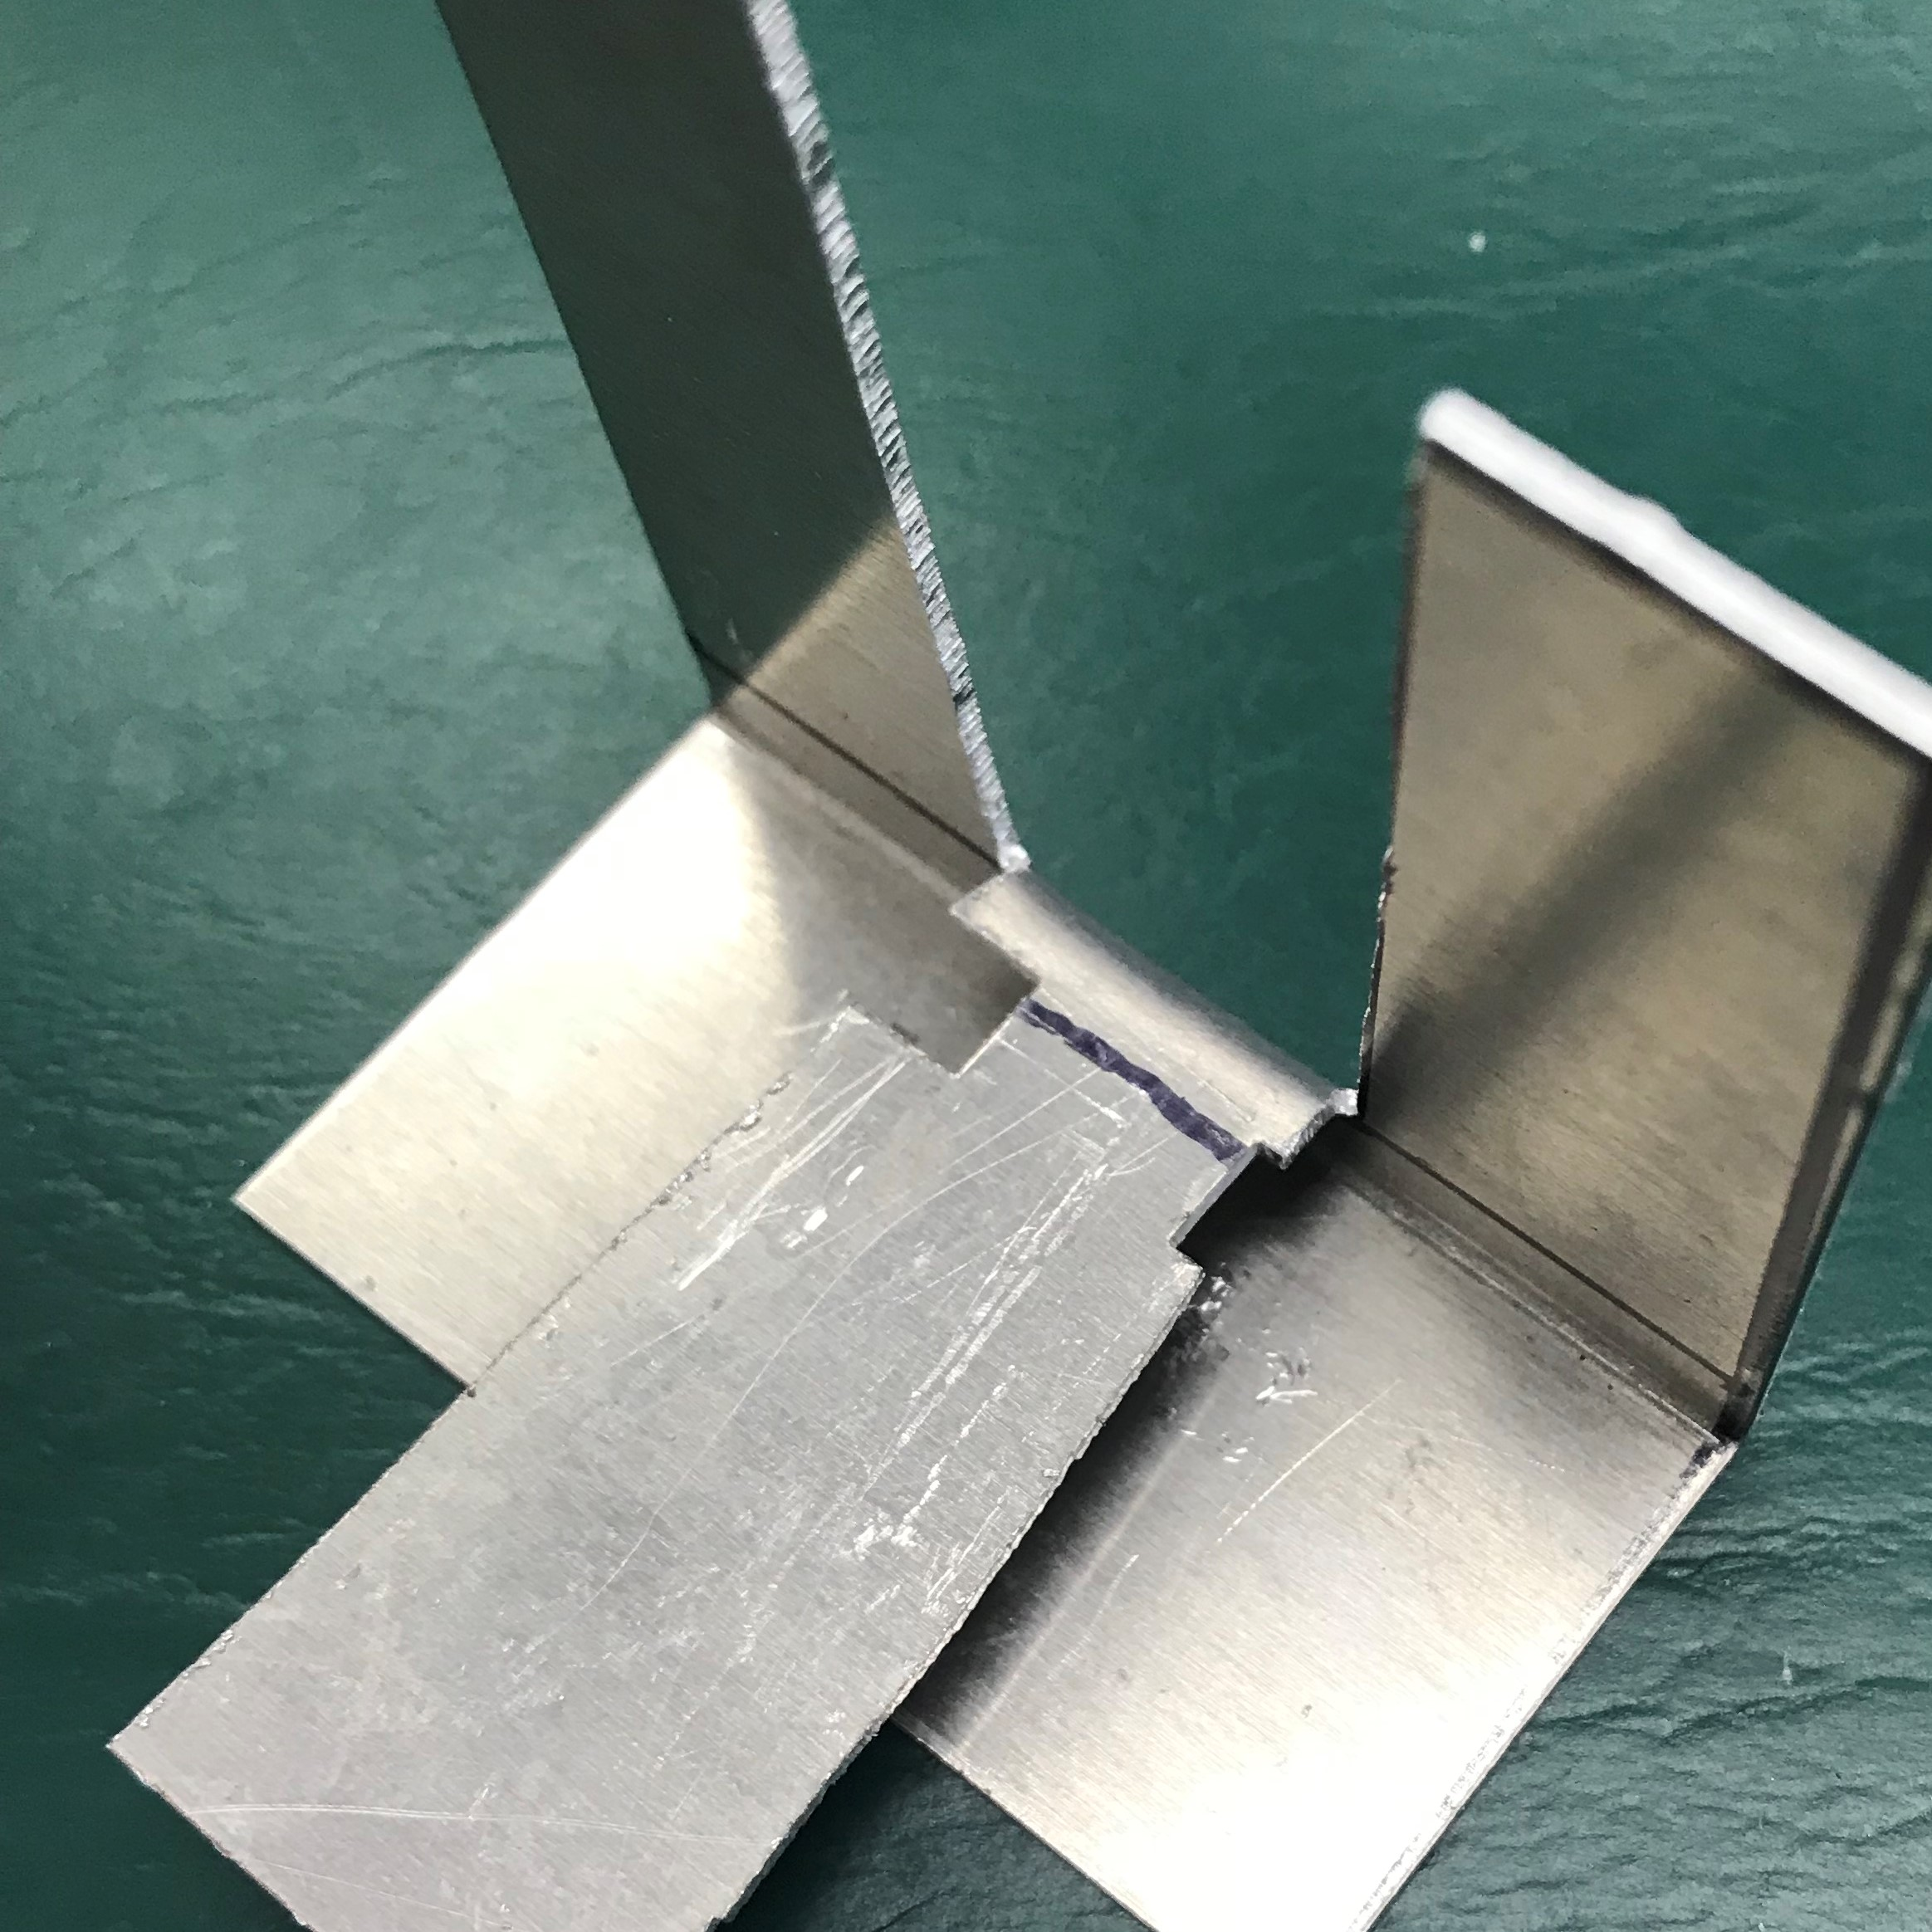
\includegraphics[width=.13\textwidth]{Design_Overview/timephoto13.jpeg}
\end{center}
\begin{center}
        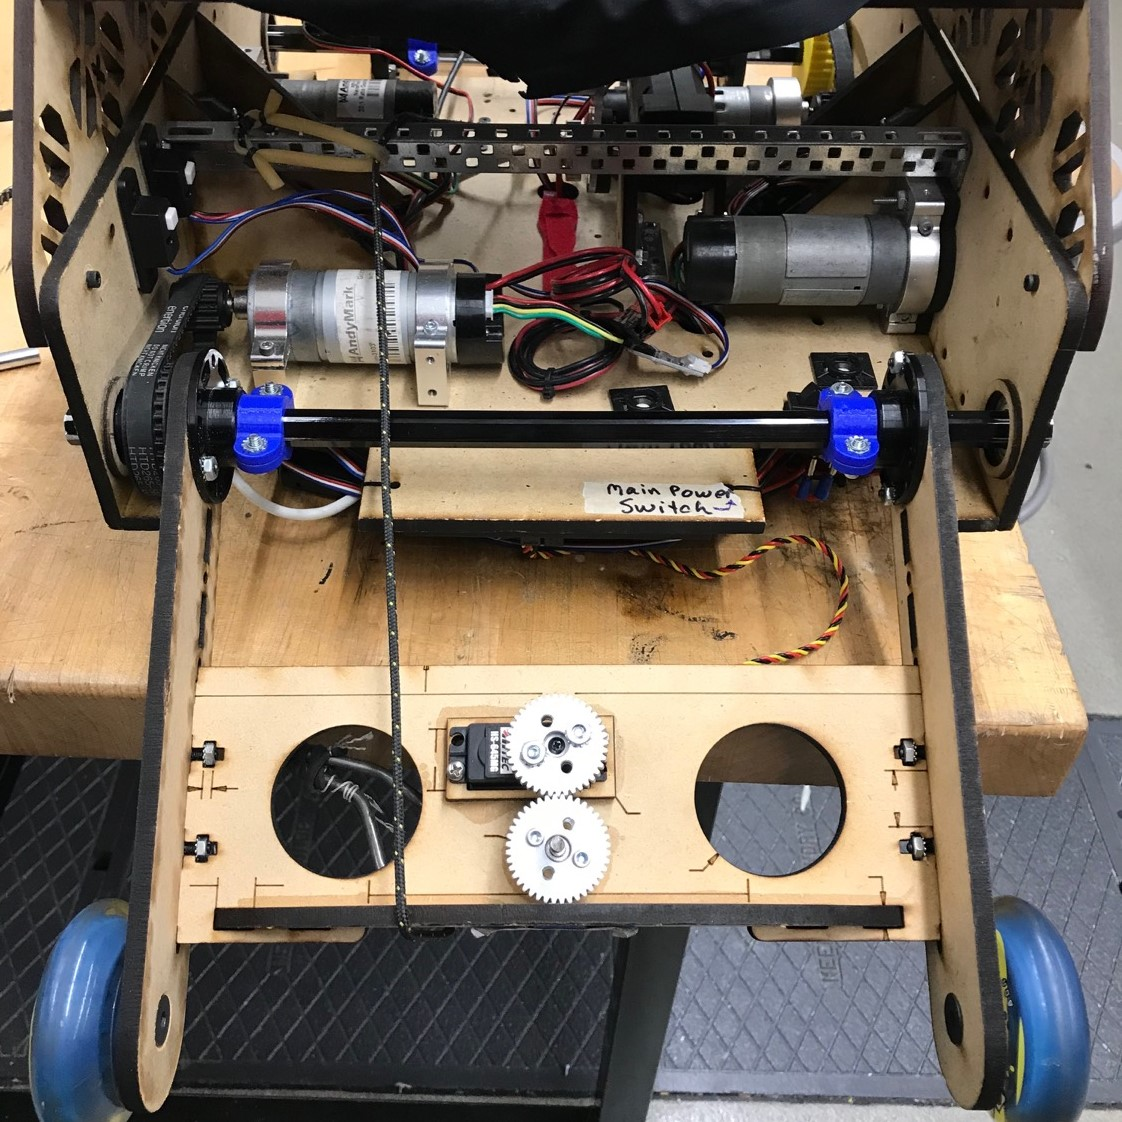
\includegraphics[width=.13\textwidth]{Design_Overview/timephoto14.jpg}
\end{center}
\begin{center}
        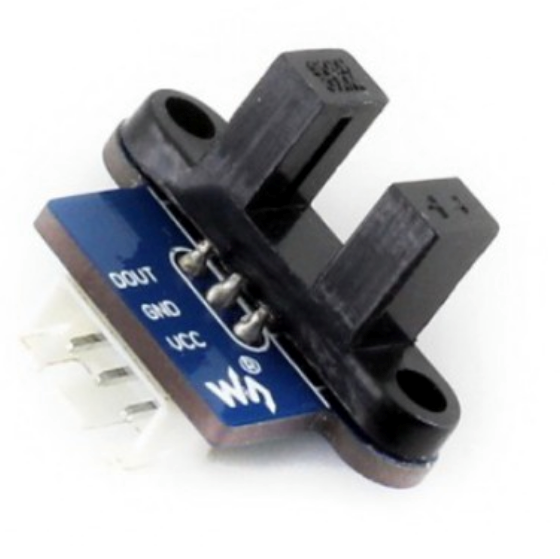
\includegraphics[width=.13\textwidth]{Design_Overview/timephoto15.png}
\end{center}
\begin{center}
        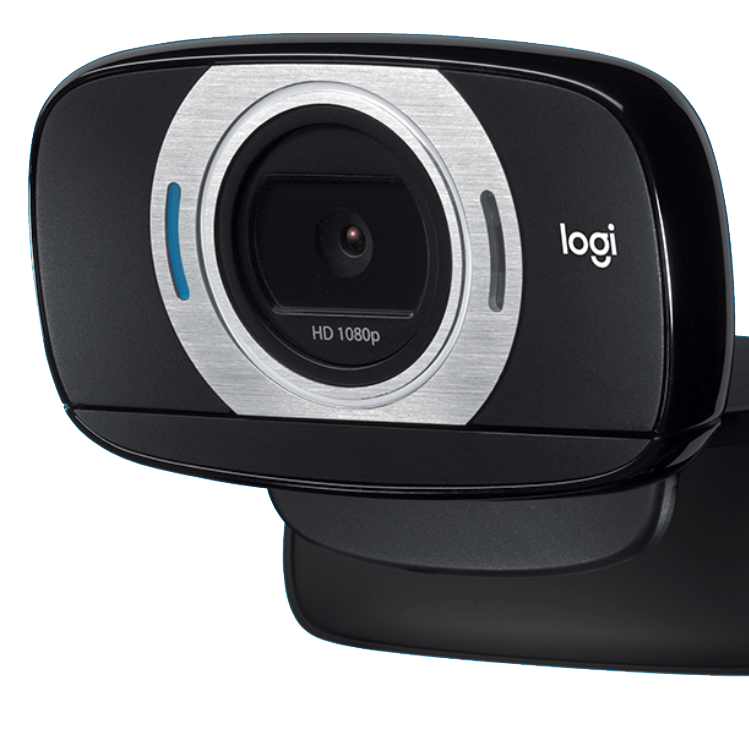
\includegraphics[width=.13\textwidth]{Design_Overview/timephoto16.png}
\end{center}
\begin{center}
        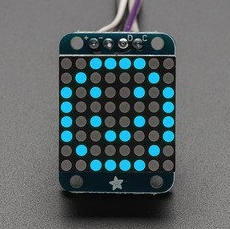
\includegraphics[width=.13\textwidth]{Design_Overview/timephoto17.png}
\end{center}
\begin{center}
        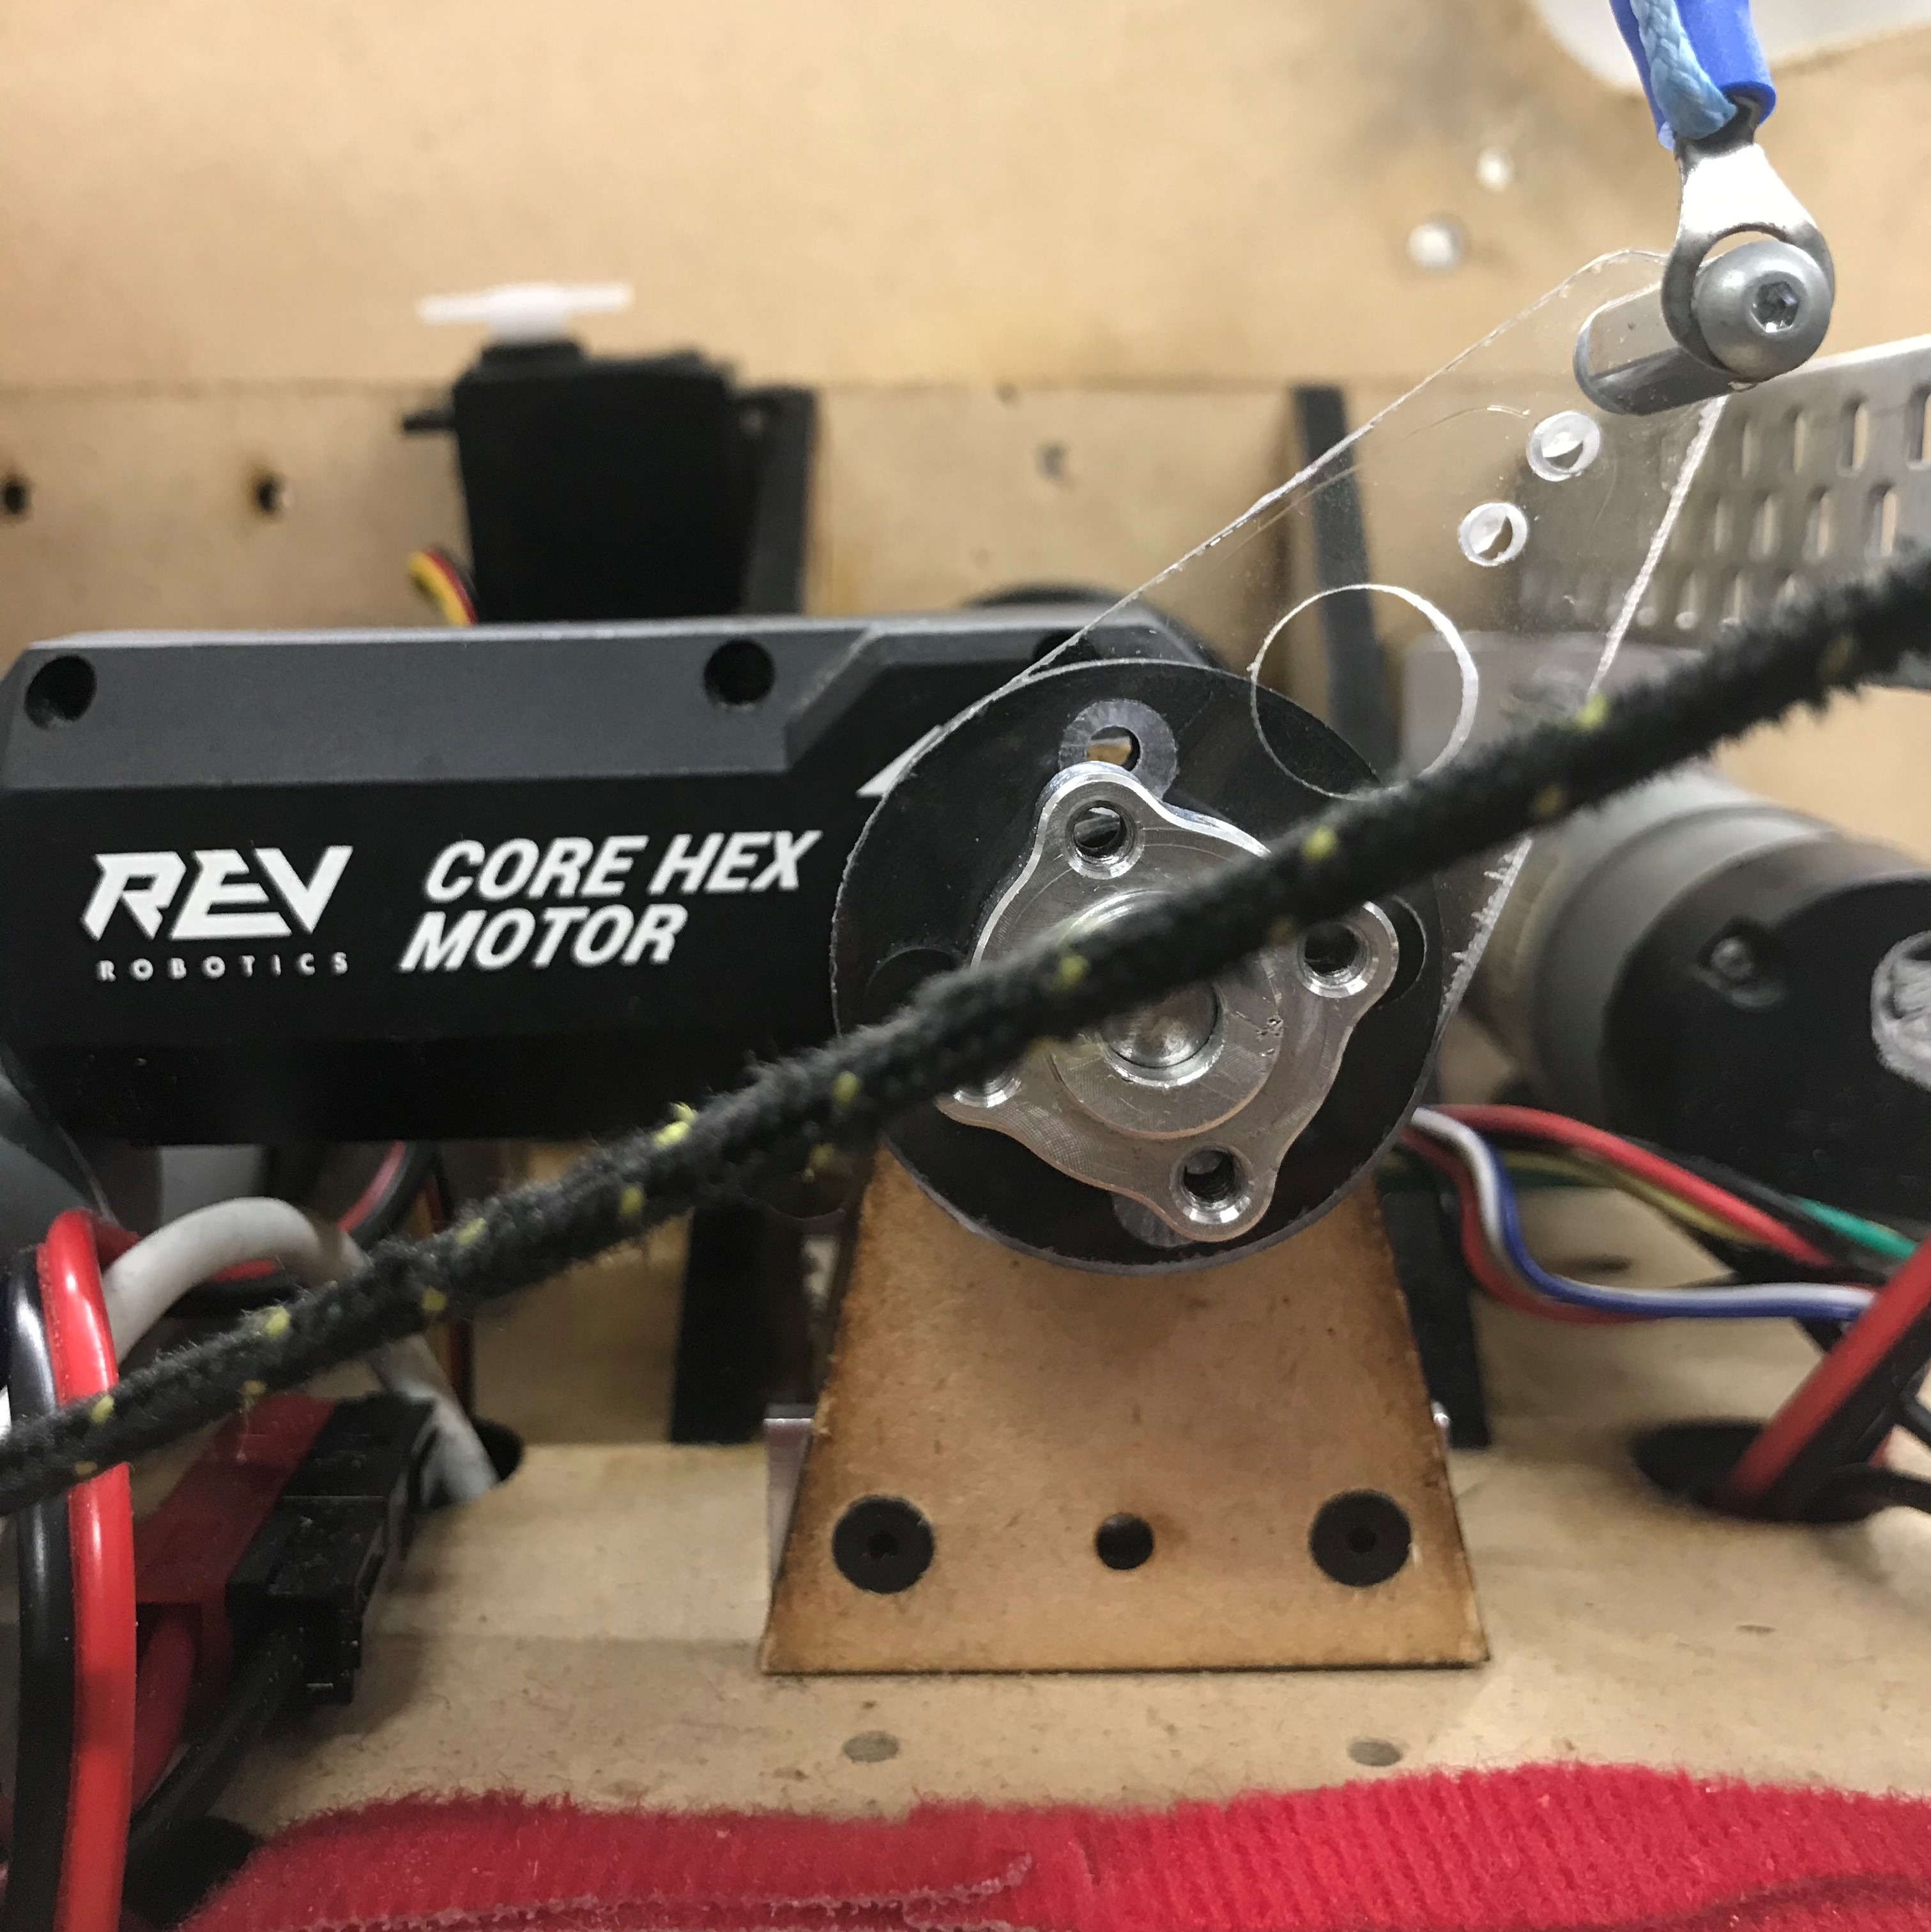
\includegraphics[width=.13\textwidth]{Design_Overview/timephoto18.jpg}
\end{center}
\begin{center}
        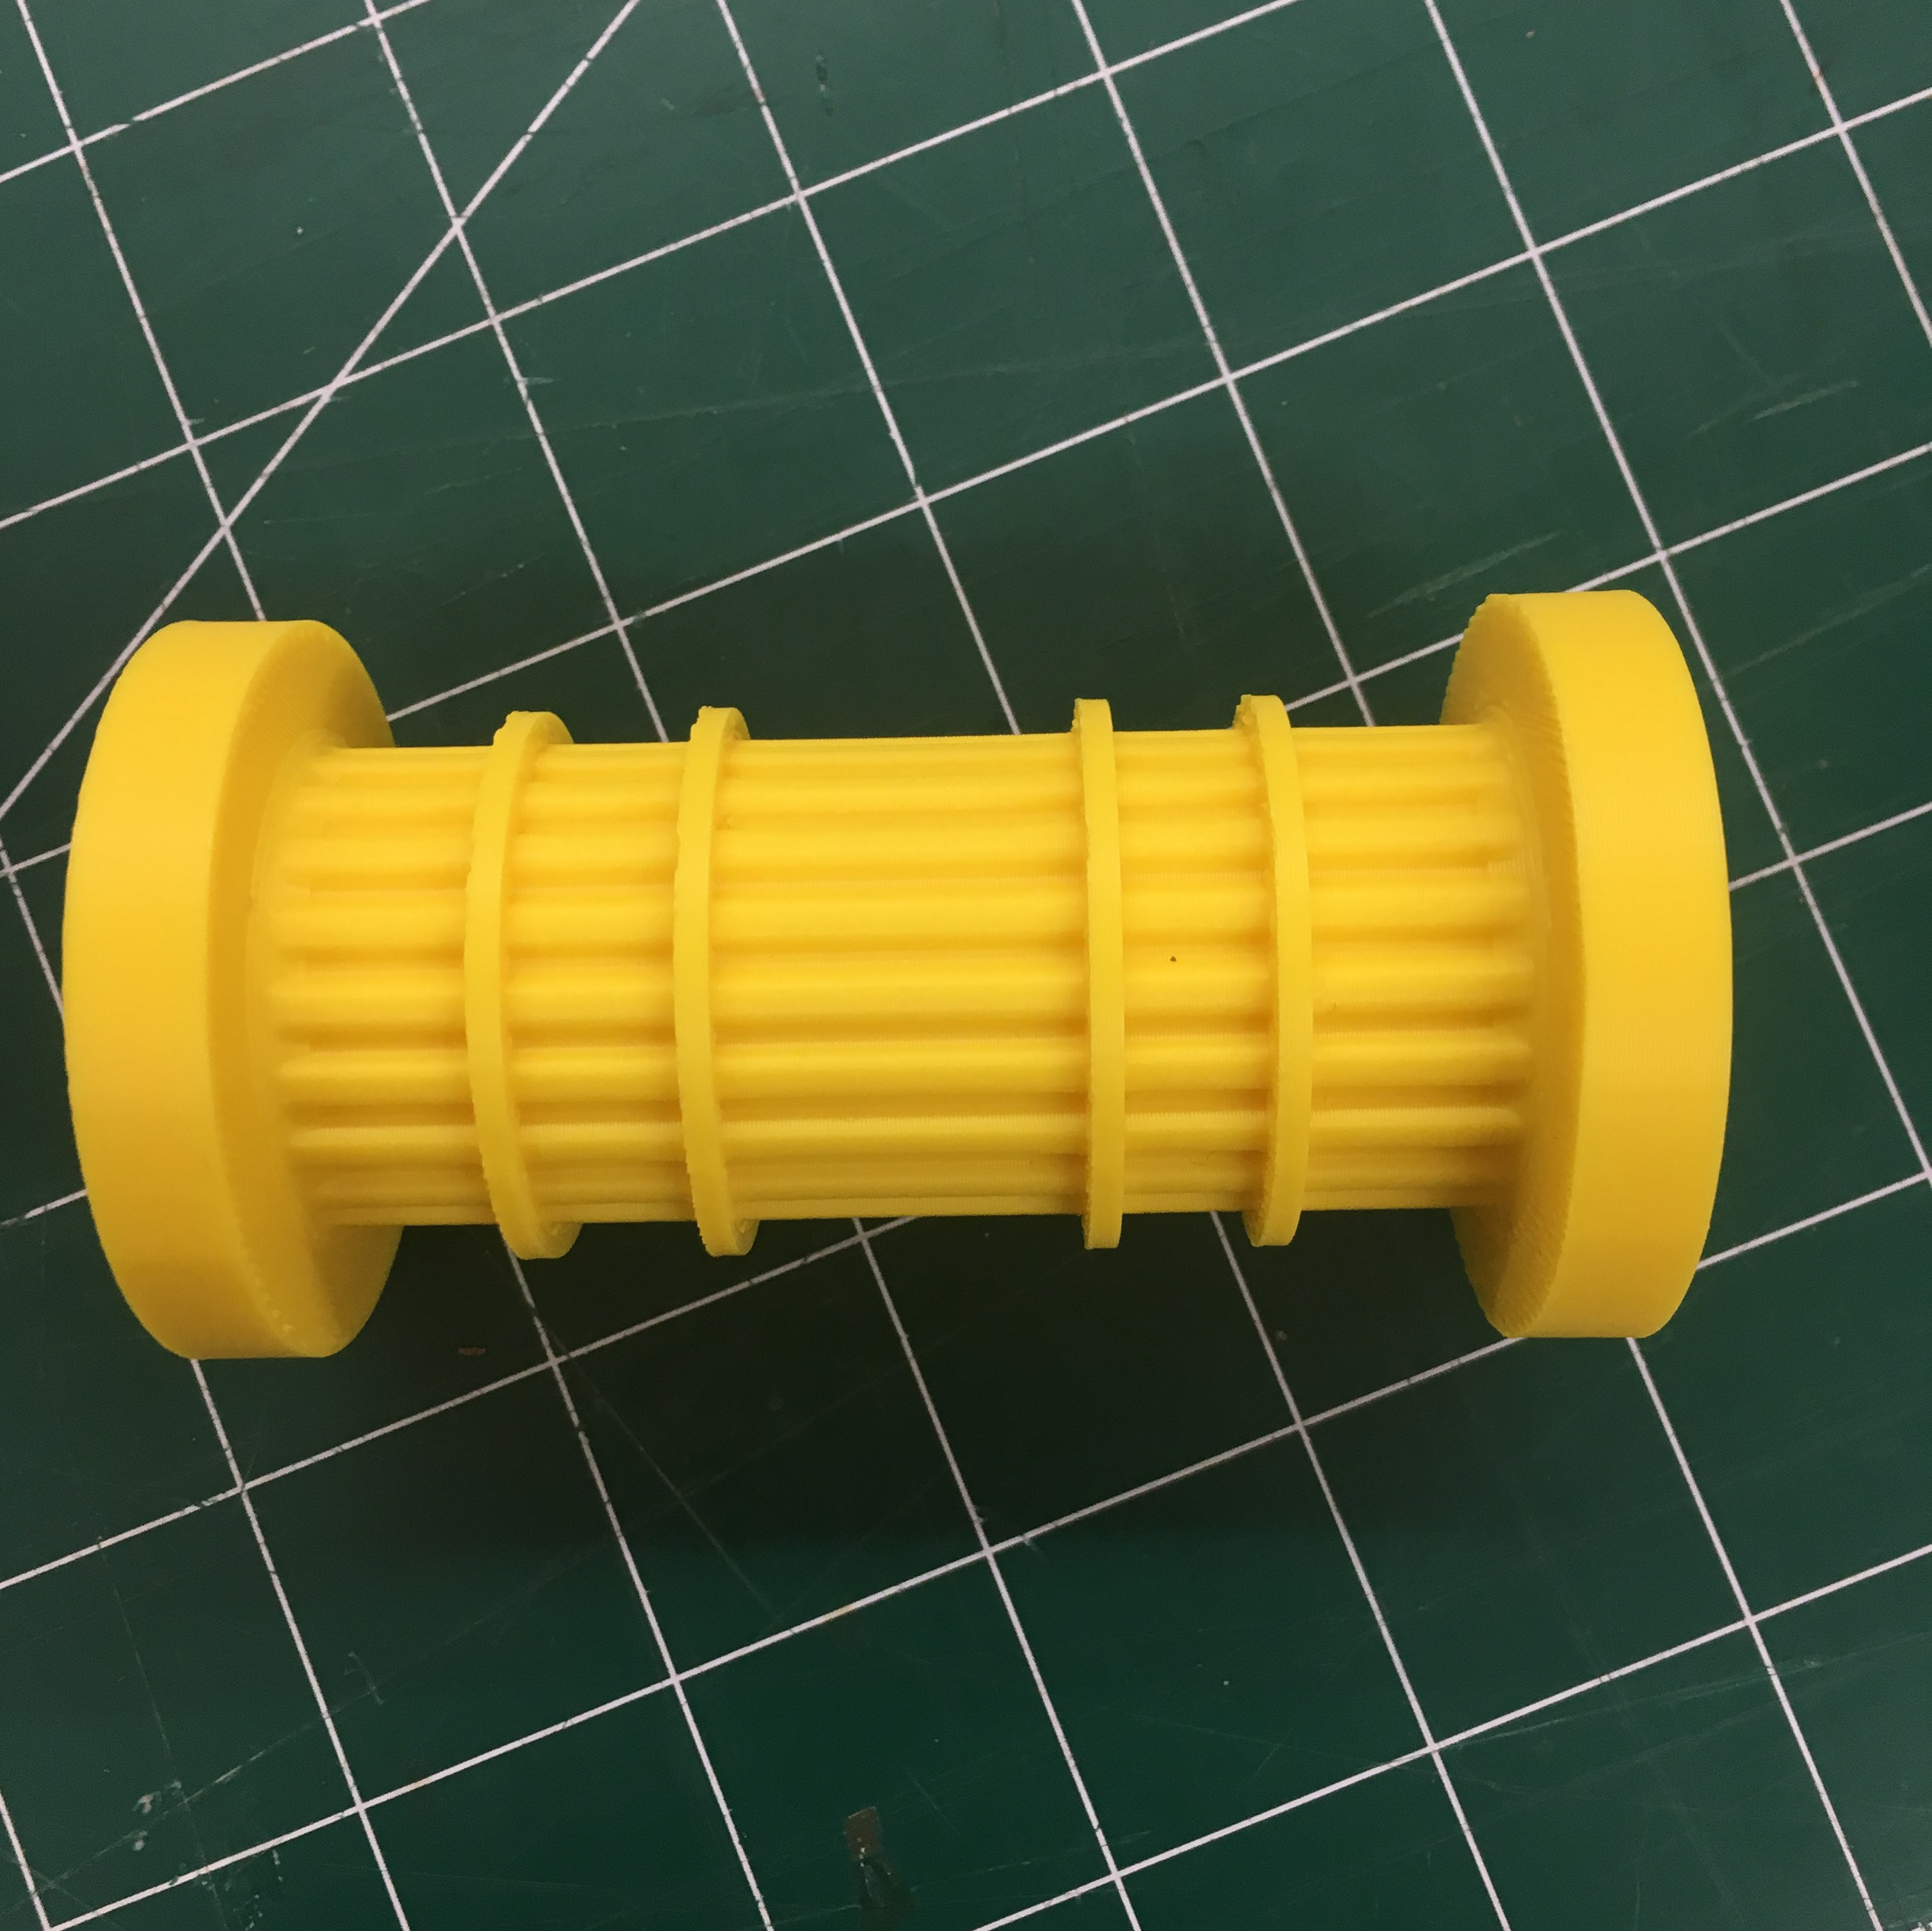
\includegraphics[width=.13\textwidth]{Design_Overview/timephoto19.png}
\end{center}


\end{multicols}